\documentclass[UTF8]{ctexart}
\usepackage{graphicx} % Required for inserting images

\title{一亿以内素数}
\author{BrightMoon}
\date{May 2024}

\begin{document}

\maketitle

\section{程序截图}
我使用了欧拉筛法。程序的外层循环是和素数配对的那个数,记作$y$。截图参考图\ref{fig:enter-label}和\ref{fig:label}
\begin{enumerate}
\item 分支一,对应$y$是素数的情况;分支二,对应$y$是合数的情况。
\item 对于分支一,首先更新已有素数表$\{ x_1,...,x_s\}\cup \{y\}$ ;分支二,无需更新。
\item 然后用$y$和已知素数$\{x_1,...,x_k\}$,相乘,筛去相应合数,条件是,素数$x_i$不超过$y$的最小质因子。

\end{enumerate}
\section{运行结果}
不计文件写入保存时间,用时2.798秒。参考图\ref{fig:entr-label}。
得到的素数写入“一亿以内质数表.txt”文本文件中。参考图\ref{fig:ener-label}和\ref{fig:ente-label}。
\begin{figure}
    \centering
    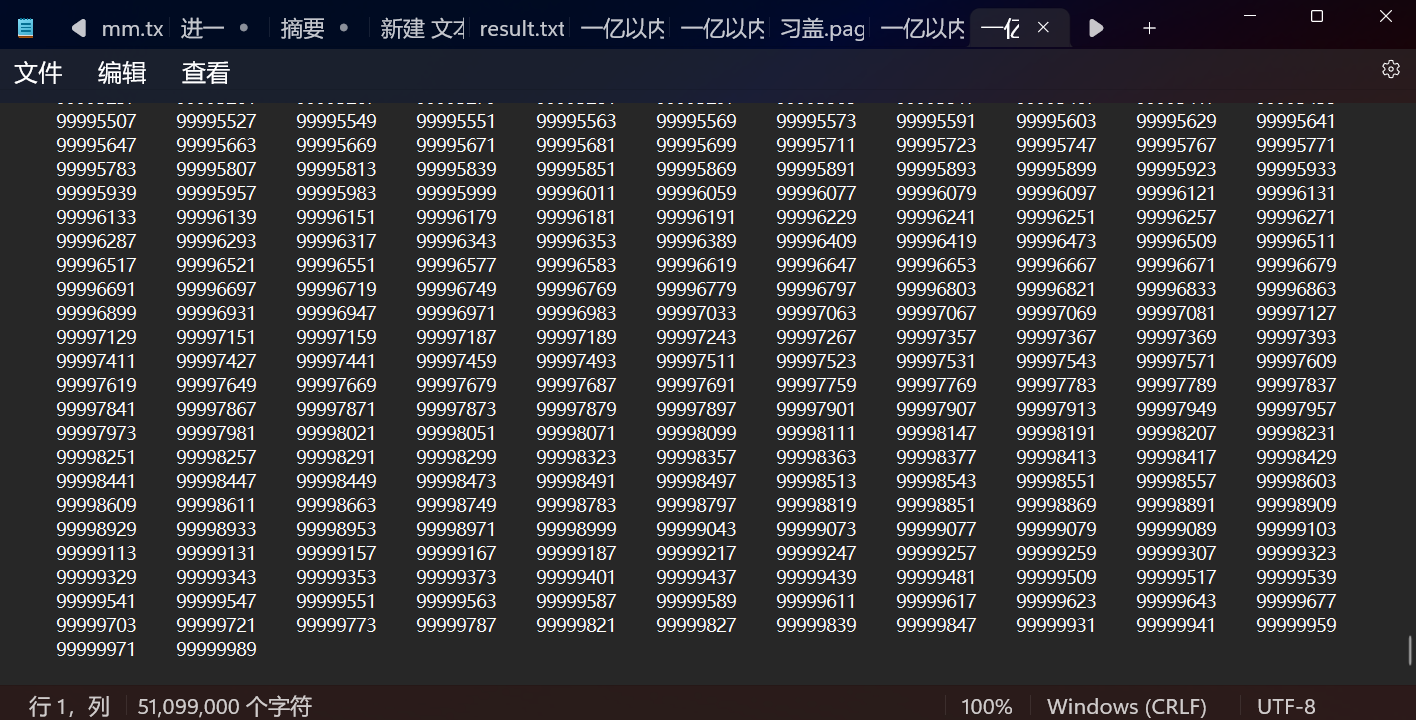
\includegraphics[width=1\linewidth]{im.png}
    \caption{质数表末端}
    \label{fig:ente-label}
\end{figure}
\begin{figure}
    \centering
    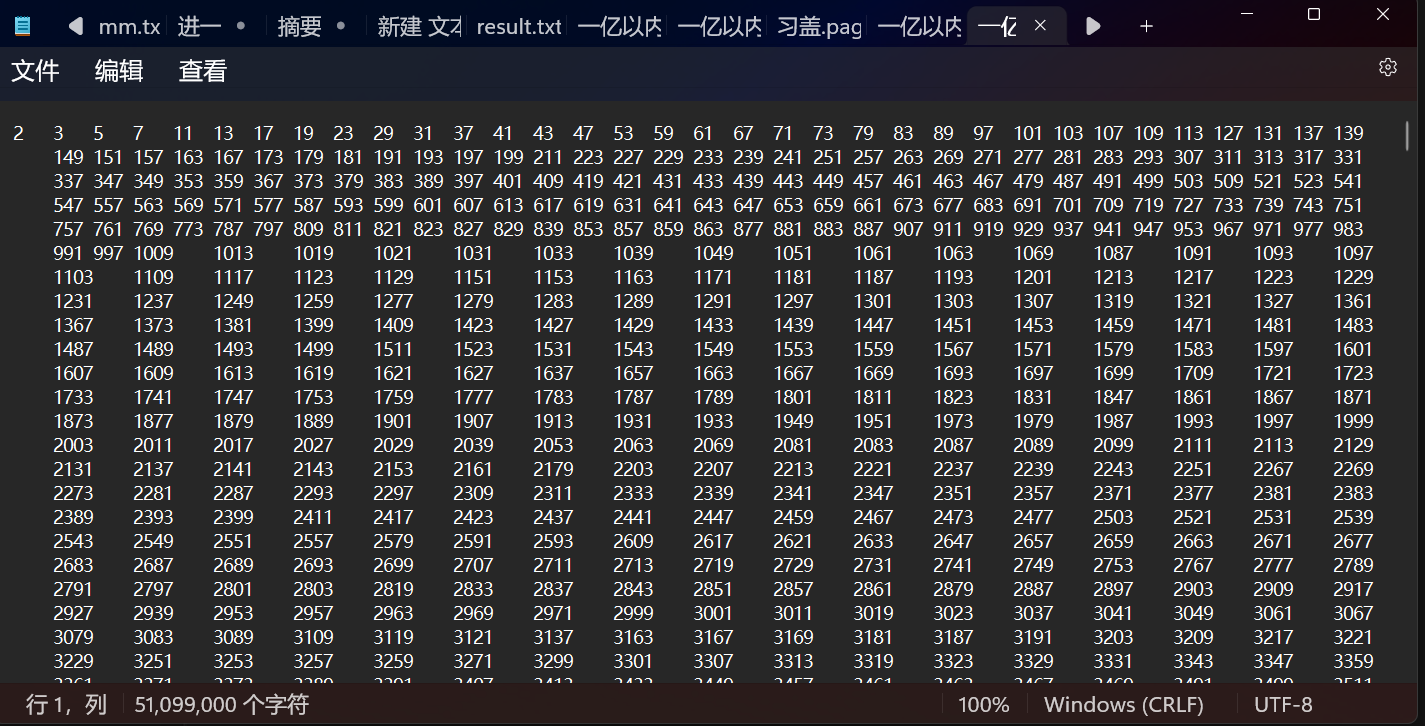
\includegraphics[width=1\linewidth]{image.png}
    \caption{质数表开头}
    \label{fig:ener-label}
\end{figure}
\begin{figure}
    \centering
    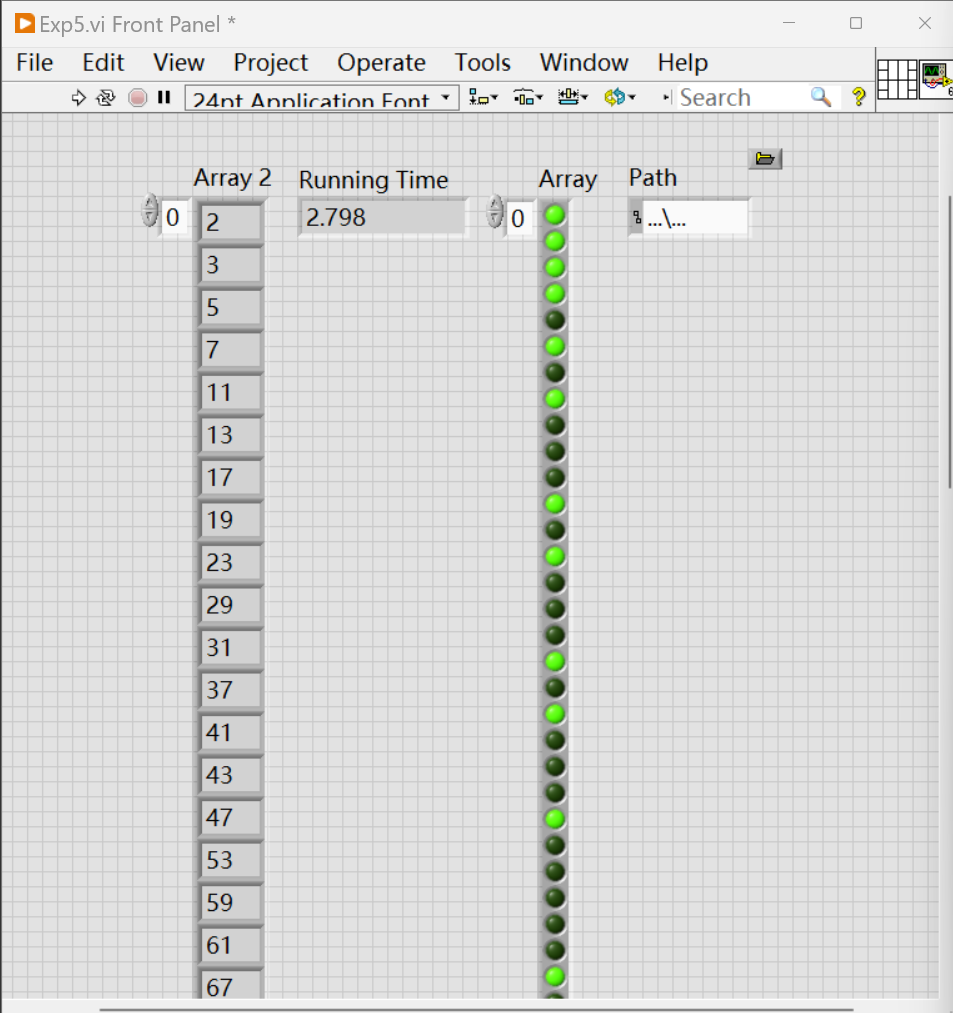
\includegraphics[width=1\linewidth]{运行效果.png}
    \caption{运行结果}
    \label{fig:entr-label}
\end{figure}

\begin{figure}
    \centering
    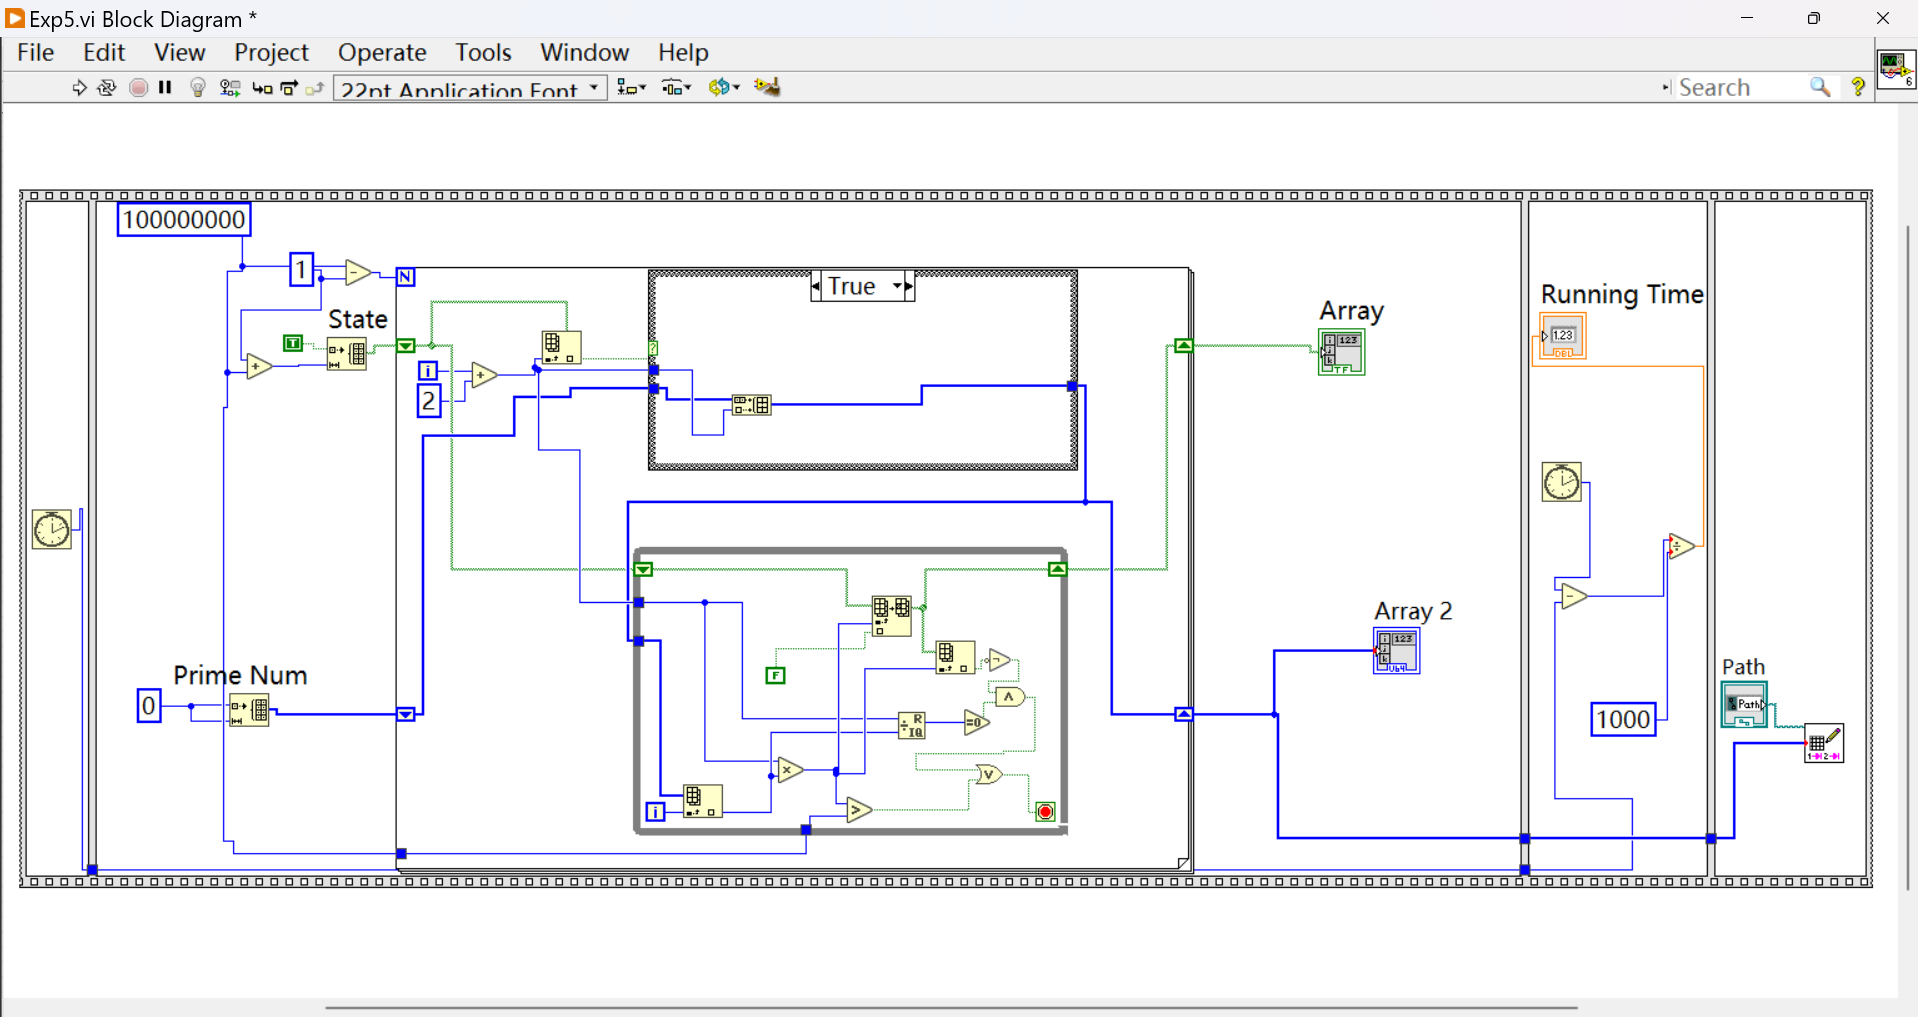
\includegraphics[width=1\linewidth]{LabView代码截图.png}
    \caption{分支一}
    \label{fig:enter-label}
\end{figure}

\begin{figure}
    \centering
    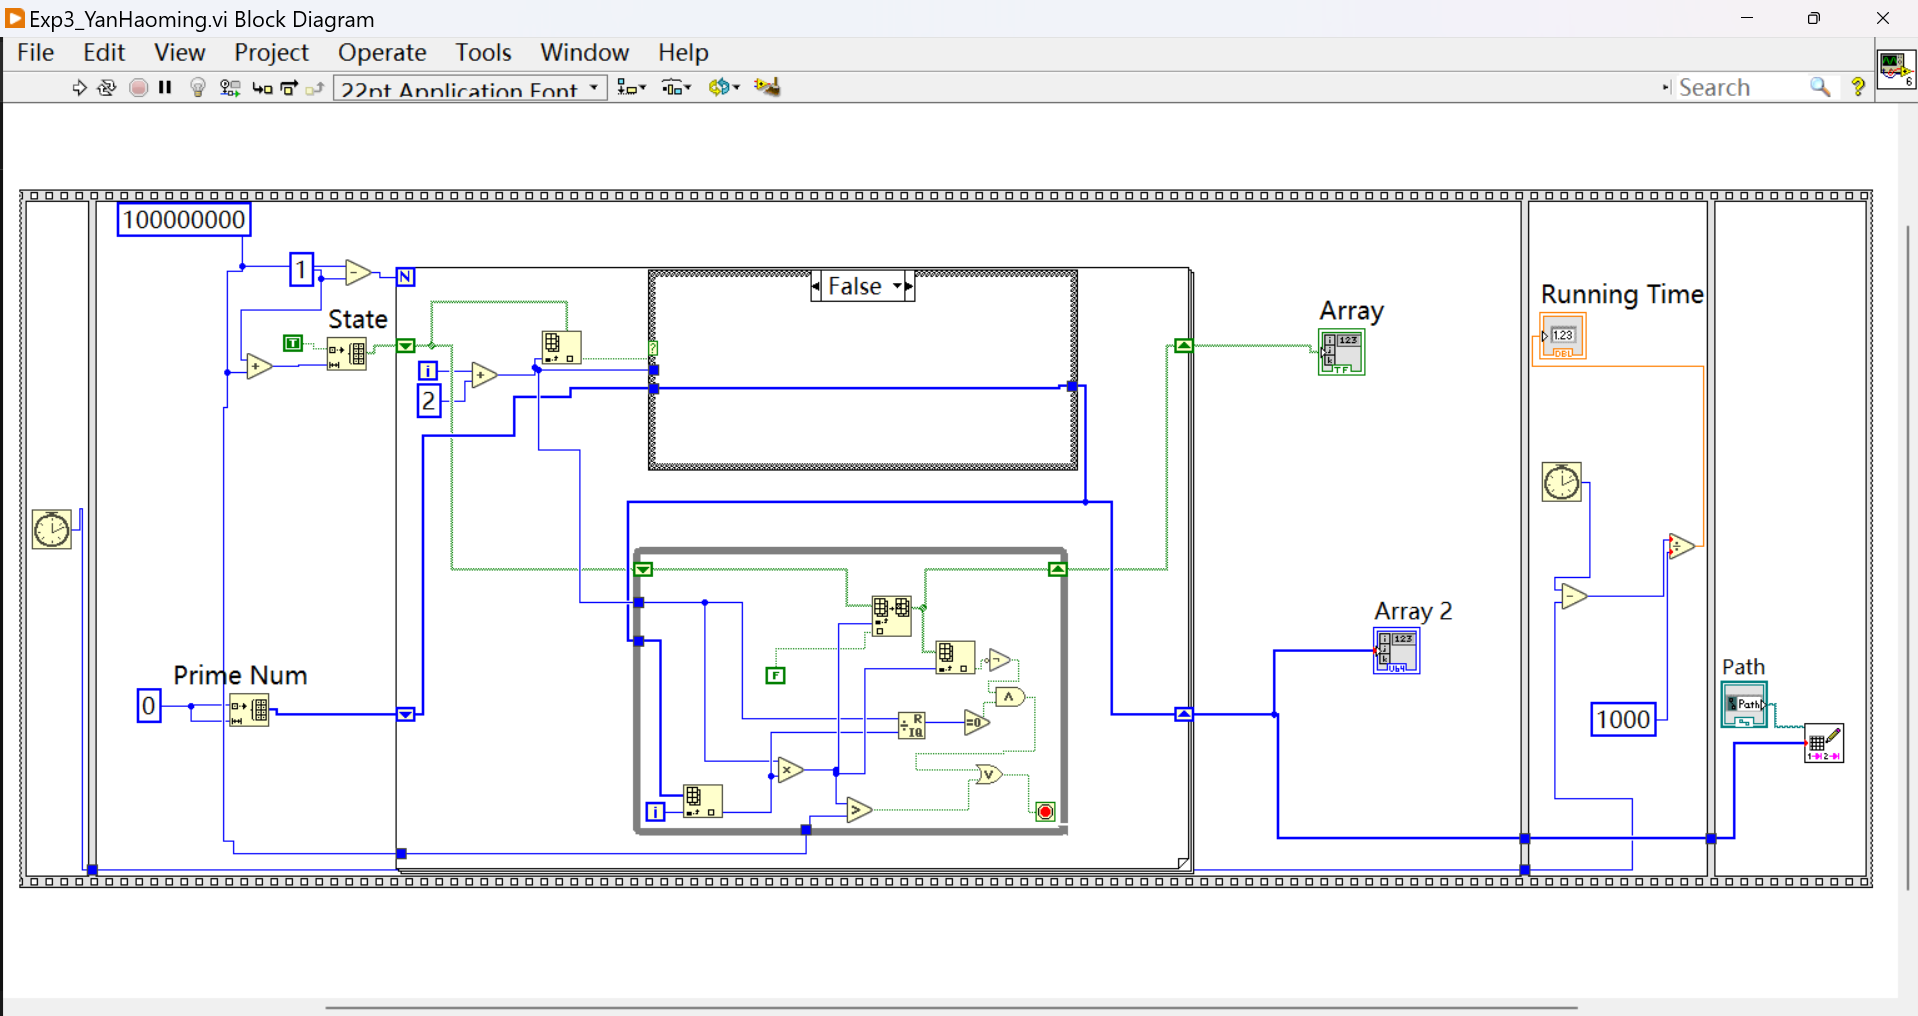
\includegraphics[width=1\linewidth]{LabView代码截图2.png}
    \caption{分支二}
    \label{fig:label}
\end{figure}
\end{document}
